\chapter{Project Design}
\section{System Architecture}

The system consists of two main components, as shown in Figure~\ref{fig:ux-flow}. The first is the Flutter application, which is installed on the user's smartphone. On the first run, it will create a local SQLite database with the required tables. Whenever a user logs in or navigates to a page, it will send a request for data to the second component, the server. It is composed of configuration and transformation modules. The former is responsible for providing the YAML configuration file in the transformation application. Because both use Spring Cloud Config, the transformation application does not need to be restarted when the config changes. Each time it is updated, the configuration server will pick up the changes and serve the updated content. Now beans from the client that were using the configuration must be refreshed. A simple way to do this is to send a GET request to the "/ refresh" endpoint provided by the Spring Boot Actuator.

\begin{figure}[htb]
    \centering
    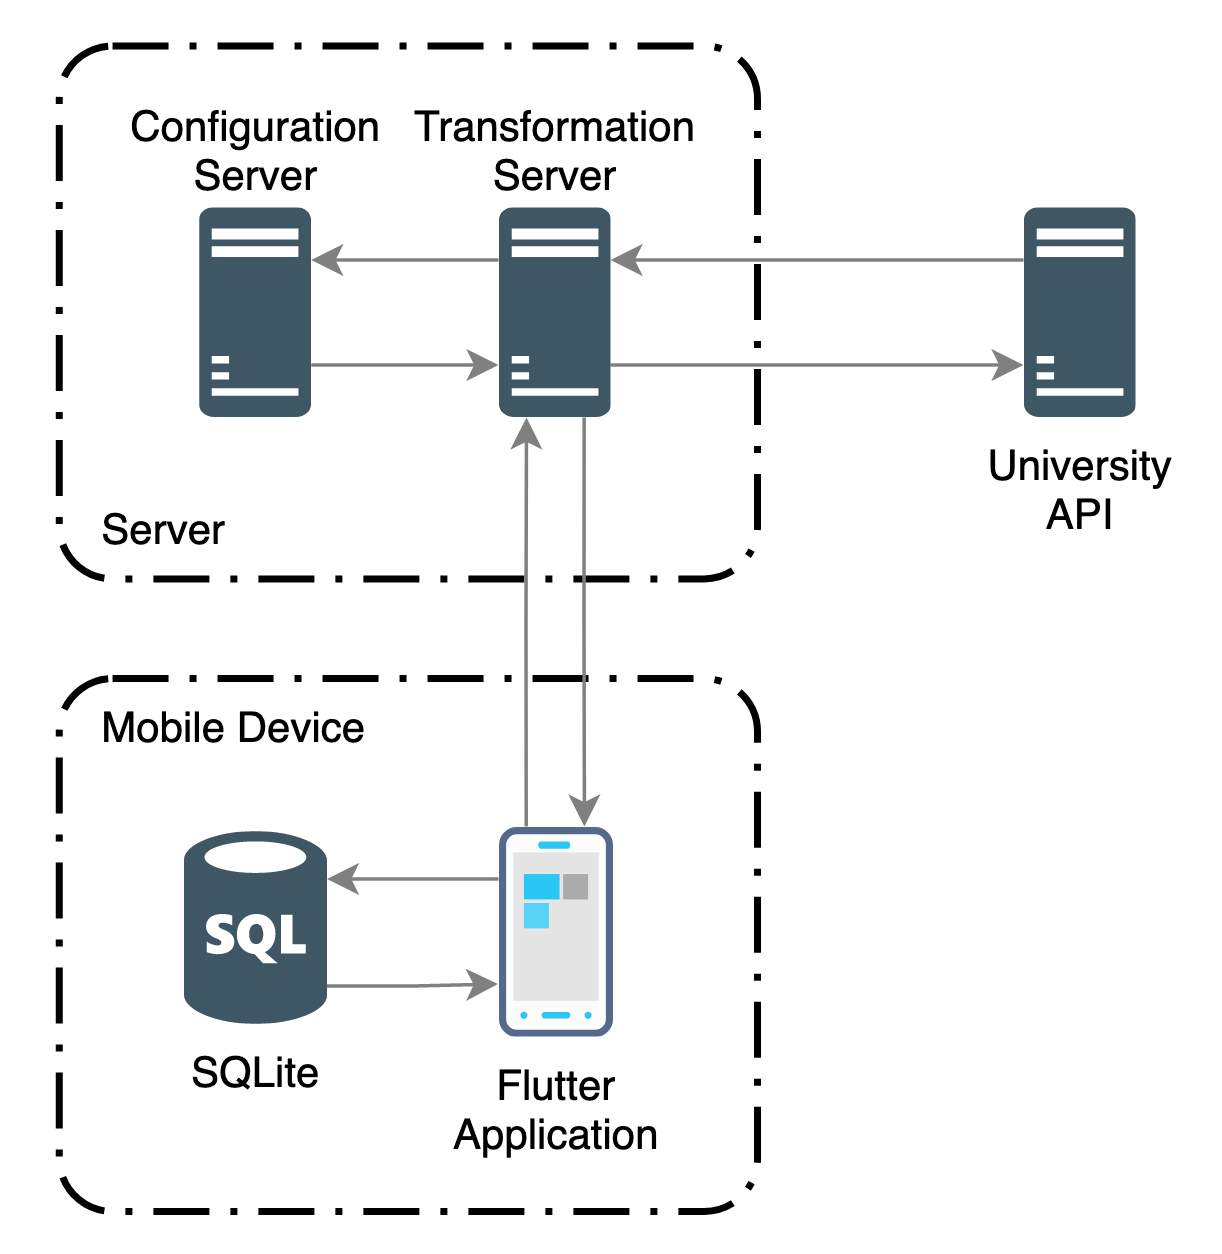
\includegraphics[width=0.55\textwidth]{fig03/system_architecture.png}
    \caption{System architecture}
    \label{fig:sys-architecture}
\end{figure}

When the transformation server receives a request, for example from Listing~\ref{list:login-request}, it reads the university and searches for a configuration for this particular institution.
\begin{lstlisting}[label=list:login-request,caption=Sample calendar request, basicstyle=\footnotesize\ttfamily]
{
    "username": "pwr123456",
    "university": "pwr",
    "startDate": "2020-01-01T00:00:00.000",
    "endDate": "2020-02-01T00:00:00.000",
},
\end{lstlisting}

A sample YAML configuration for calendars is shown in Listing~\ref{list:calendar-config}. It contains an object with the name "pwr" and a configuration for this university. Every config entry has to contain a name, address, a specification for Jolt transformation for request and response.

\begin{lstlisting}[label=list:calendar-config,caption=Sample YAML configuration for calendars, basicstyle=\footnotesize\ttfamily, breaklines=true]
calendars:
    - name: 'pwr'
      address: 'http://localhost:1080/calendars'
      request: '[{"operation": "shift","spec": {"username": "user","studentNumber": "indeks","startDate": "date.start","endDate": "date.end"}}]'
      response: '[{"operation": "shift","spec": {"events": {"*": {"eventName": "events.[&1].name","room": "events.[&1].classroom","type": "events.[&1].eventType","date": {"start": "events.[&2].startDateTime","end": "events.[&2].endDateTime"},"*": "events.[&1].&"}}}}]'
\end{lstlisting}

Every transformation operation requires a specification.

% TODO - finish this

\section{Database Design}
The mobile database is very straightforward. There are five separate tables as seen in Figure~\ref{fig:erd-diagram}. All of them are created during the first run of the application. Data received from the server is stored locally in the SQLite database. Every time the application sends a successful request, information in a chosen table is updated with new data. If there is no connection to the Internet, the app takes already stored details from the database instead of sending a request. Thanks to it, users can have constant access to data.
\begin{figure}[htb]
    \centering
    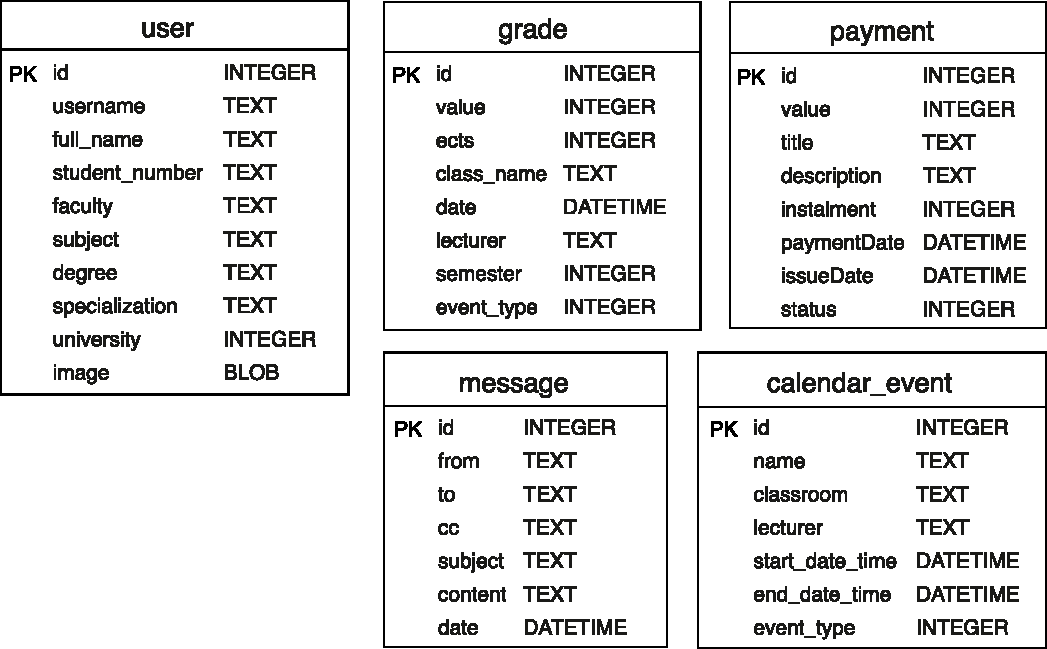
\includegraphics[scale=0.7]{fig03/erd_diagram-01.pdf}
    \caption{ERD diagram for the mobile database}
    \label{fig:erd-diagram}
\end{figure}

\section{User Interface Design}

% TODO - ask what about Sketch, do I need a link or sth?
All mobile applications should be easy to use and intuitive. In our app, we used Material Design created by Google. It is also a part of the Flutter toolkit. To make the development quicker and easier, we created wireframes for all the main views of the application. To create them, we worked with a tool called Sketch, which is simple to use and has a lot of available libraries.

There are seven main screens available. All of them are shown in Figure~\ref{fig:ux-flow}. The first screen is a login screen. After users enter the correct login and password, they are redirected to the homepage. There they can see their profile info and news for their university and faculty. On the bottom, there is a navigation bar from which they can get access to an additional four pages. The first of the is the calendar page where they can see their schedule. The next one is the grades page where they can view all their grades. After it, there is the messages page where users can access their e-mails and go to the messages details page. The last one is the finances page. It allows users to see all of their payments.

% TO DO: poprawić rysunek, by był w układzie jak ten poniżej
\begin{figure}[htb]
    \centering
    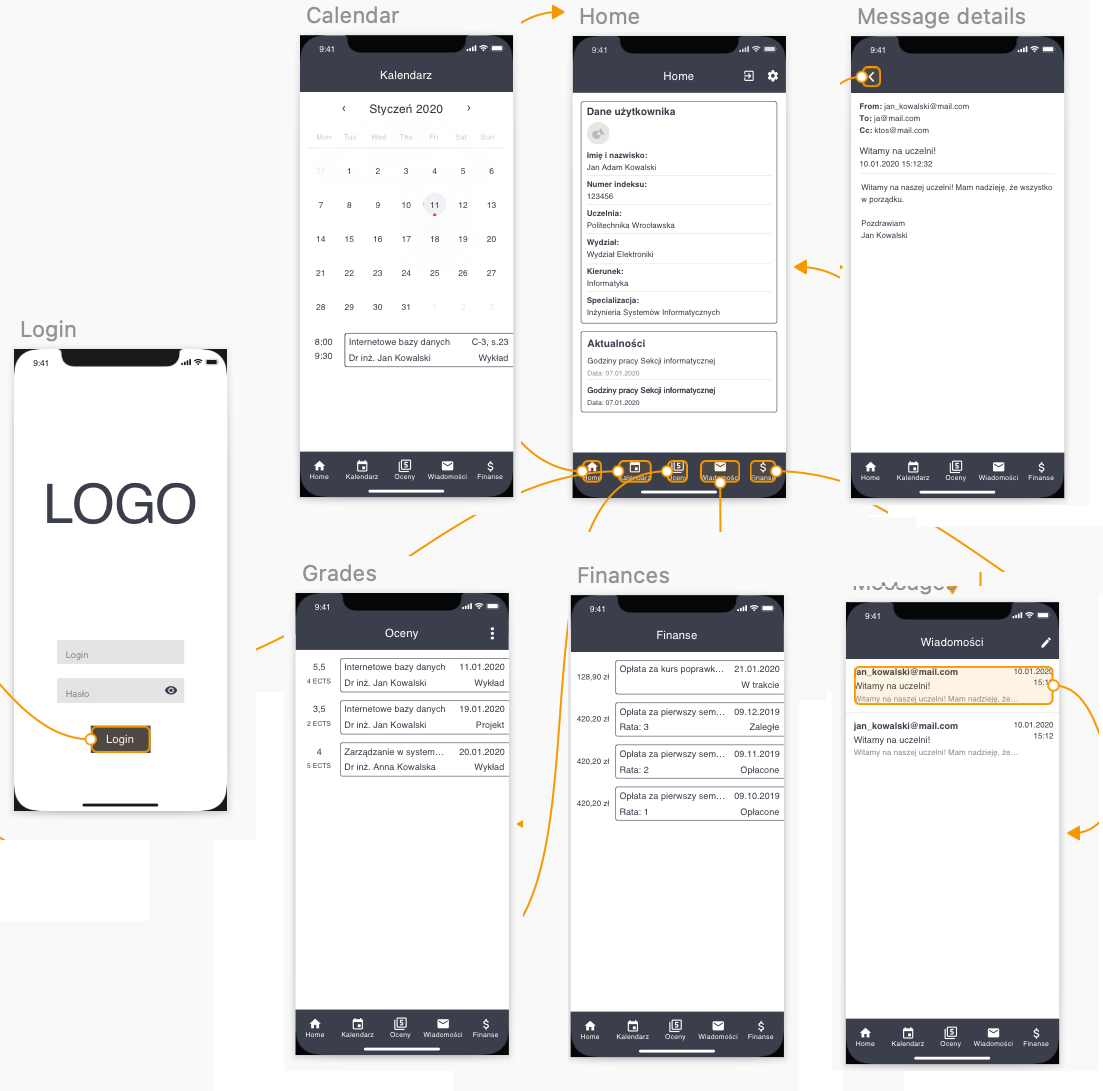
\includegraphics[width=0.83\textwidth]{fig03/mobile_ux_flow-1-2x3.png}
    \caption{Mobile UX flow}
    \label{fig:ux-flow}
\end{figure}

The first screen that is presented to users is the login screen. It is shown in Figure~\ref{fig:login-home}. There is a big logo of the application in the middle of the view. There are also two input boxes on the bottom of the screen with a button to submit them. If the data provided is incorrect, users are presented with a red error snack bar.

The home screen, also presented in Figure~\ref{fig:login-home}, is the main page of the application. It contains profile info with the logged-in student's data. There is also a news feed section where users can access news from their university or faculty, depending on the configuration. In the top right corner of the screen, there are two icons. The first one allows users to log out of the application. By clicking on the next one, users can access the settings.

\begin{figure}[htb]
    \centering
    \begin{tabular}{@{}ll@{}}
        a) & b) \\
        {\setlength{\fboxsep}{0pt}\setlength{\fboxrule}{1pt}\fbox{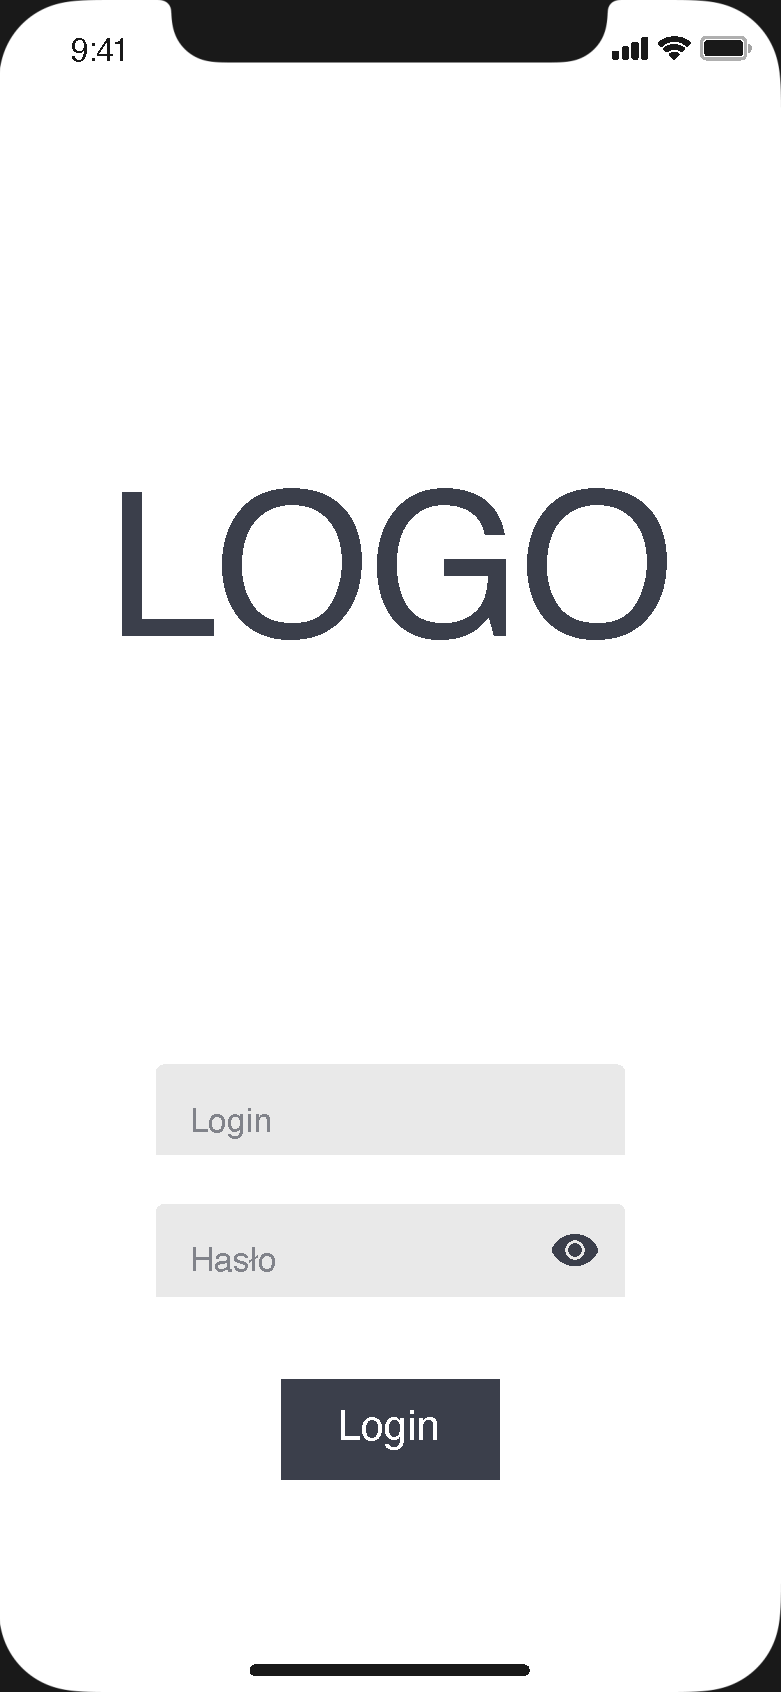
\includegraphics[page=1,width=0.300\textwidth]{fig03/jsos_helper_wireframe.pdf}}} &
        {\setlength{\fboxsep}{0pt}\setlength{\fboxrule}{1pt}\fbox{\includegraphics[page=7,width=0.300\textwidth]{fig03/jsos_helper_wireframe.pdf}}} \\
    \end{tabular}
    \caption{Wireframes: a) login page, b) homepage} \label{fig:login-home}
\end{figure}

The calendar page shown in Figure~\ref{fig:calendar-finances-grades} contains a calendar with the list of dates. If a date is a holiday, there is an indicator shown in the right top corner of the container. An indicator at the bottom of the container informs users that they have some lectures during the selected date.
When users click on a date, a list of classes is shown under the calendar. Every row contains the start and the end time of the event, its name, university teacher, classroom, and a type of the event.

The next screen presented in Figure~\ref{fig:calendar-finances-grades} is the finances page. It is composed of a list of payments with their details. Every entry includes an amount, status, name, and the date of the payment's issue. Some of them also contain an installment number.

The last screen from Figure~\ref{fig:calendar-finances-grades} consists of a grades list. Each entry contains a grade, number of ECTS credits, course name, type and university teacher, and issuing date. The icon in the top right corner allows users to calculate their average grade for a semester or the whole studies.

\begin{figure}[htb]
    \centering
    \begin{tabular}{@{}lll@{}}
        a) & b) & c) \\
        {\setlength{\fboxsep}{0pt}\setlength{\fboxrule}{1pt}\fbox{\includegraphics[page=2,width=0.300\textwidth]{fig03/jsos_helper_wireframe.pdf}}} &
        {\setlength{\fboxsep}{0pt}\setlength{\fboxrule}{1pt}\fbox{\includegraphics[page=6,width=0.300\textwidth]{fig03/jsos_helper_wireframe.pdf}}} &
        {\setlength{\fboxsep}{0pt}\setlength{\fboxrule}{1pt}\fbox{\includegraphics[page=3,width=0.300\textwidth]{fig03/jsos_helper_wireframe.pdf}}} \\
    \end{tabular}
    \caption{Wireframes: a) calendar page, b) finances page, c) the grades page} \label{fig:calendar-finances-grades}
\end{figure}

The two last screens shown in Figure~\ref{fig:messages-and-details} present a list of messages and their details. The first page is composed of the email sender, topic, date received, and partial contents. When customers click on an email, they are redirected to the details page where the full contents of the email are shown along with Cc'd recipients. After users have read the email, they can get back to the emails list by clicking an arrow on the top of the screen. In the top right corner of the screen, there is an icon that is shown only when the user university's API allows for sending messages.

\begin{figure}[htb]
    \centering
    \begin{tabular}{@{}ll@{}}
        a) & b) \\
        {\setlength{\fboxsep}{0pt}\setlength{\fboxrule}{1pt}\fbox{\includegraphics[page=4,width=0.300\textwidth]{fig03/jsos_helper_wireframe.pdf}}} &
        {\setlength{\fboxsep}{0pt}\setlength{\fboxrule}{1pt}\fbox{\includegraphics[page=5,width=0.300\textwidth]{fig03/jsos_helper_wireframe.pdf}}} \\
            \end{tabular}
    \caption{Wireframes: a) messages page, b) message details page} \label{fig:messages-and-details}
\end{figure}
